\documentclass[11pt,letterpaper,twoside]{book}

\usepackage[margin=0.75in]{geometry}
\usepackage{lipsum}
\usepackage{graphicx}
\usepackage{amsmath}

\begin{document}

\tableofcontents

\chapter{First Chapter}

\lipsum[1-2]

\section{First Section}

\lipsum[3-5]

\subsection{Sub Section}

\lipsum[7-9]

\subsection{Another Sub Section with some math}

\lipsum[6-8]
Recall the Fourier\footnote{A footnote test} series formula\footnote{another footnote test \lipsum[1]}:
\[
f(x) = a_0 + \sum_{n = 1}^\infty \left( a_n \cos nx + b_n \sin nx \right)
\]
Where the Fourier coefficients $a_0$, $a_n$ and $b_n$ are defined by:
\[
a_0 = \frac{1}{2L} \int_{-L}^L f(x) dx  \qquad
a_n = \frac{1}{L}  \int_{-L}^L f(x) \cos \left( \frac{n\pi x}{L} \right) dx \qquad
b_n = \frac{1}{L}  \int_{-L}^L f(x) \sin \left( \frac{n\pi x}{L} \right) dx 
\]
\lipsum[33-34]

\section{Another Section with a Picture}

\lipsum[9]
\begin{figure}
\centering
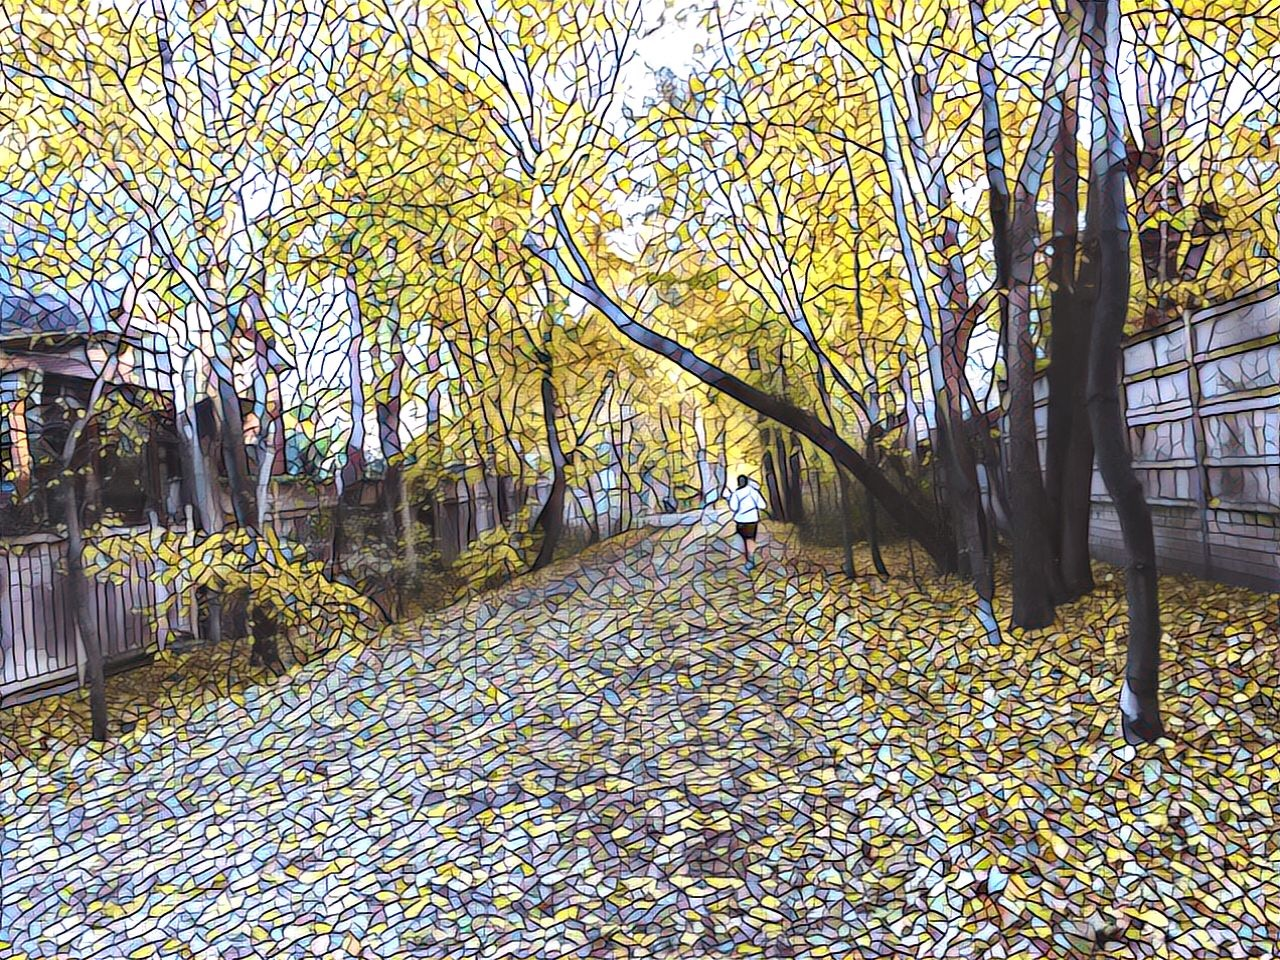
\includegraphics[width=0.5\textwidth]{TrailPic1}
\caption{\label{fig:path}A nice picture of the beltway trail}
\end{figure}

\lipsum[10-11]

\section{Another Section with more pictures}

\lipsum[12-13]

\begin{figure}
\centering

\includegraphics[width=0.4\textwidth]{BooksPic1}
\qquad

\includegraphics[width=0.4\textwidth]{BooksPic2}
\caption{\label{fig:path}Books and books}
\end{figure}

\lipsum[13-14]

\section{More Math}

\lipsum[15-16]

\[
\mathsf{Square\ Wave}(x) = \left\{ 
      \begin{array}{ll} 1, & 0 \leq x < 1 \\ 
                       -1, & 1 \leq x < 2 \end{array} \right.
\]

First we can determine $a_0$.  By inspection we can expect it to be zero, but we shall still 
figure it out for practice.  Note that $L = 1$ and we are considering the interval $[0, 2)$ instead
of $[-1, 1)$ since the function is periodic:
\begin{align*}
a_0 &= \frac{1}{2L} \int_{-L}^L f(x) dx  \\
    &= \frac{1}{2(1)} \int_{0}^{2} \mathsf{Square\ Wave}(x) dx \\
    &= \frac{1}{2} \left[ \int_0^1 (1) dx + \int_1^2 (-1) dx \right] = \frac{1}{2} \left[ \left. \vphantom{\frac{1}{2}} x\right|^1_0 - \left. \vphantom{\frac{1}{2}} x\right|^2_1 \right] \\
    &= \frac{1}{2} \left[ \vphantom{\frac{1}{2}} 1 - 0 - (2 - 1) \right] \\
    &= 0
\end{align*}

Next we shall look at $a_n$.  Again by inspection we can argue that since the function is odd that it
cosine components since those are even.  Anyways... we shall still work it out for practice.
\begin{align*}
a_n &= \frac{1}{L}  \int_{-L}^L f(x) \cos \left( \frac{n\pi x}{L} \right) dx \\
    &= \frac{1}{(1)} \int_{0}^{2} \mathsf{Square\ Wave}(x)\cos \left( \frac{n\pi x}{1} \right) dx \\ 
    &= \int_0^1 (1) \cos \left( n\pi x \right) dx + \int_1^2 (-1) \cos \left( n\pi x \right) dx \\
    &= \left. \frac{1}{n \pi} \sin \left( n\pi x \right)\right|^1_0 -  \left. \frac{1}{n \pi} \sin \left( n\pi x \right)\right|^2_1 \\
    &= \frac{1}{n \pi} \left( \vphantom{\frac{1}{2}} \sin ( n\pi) - \sin(0) \right) - \frac{1}{n \pi} \left( \vphantom{\frac{1}{2}} \sin (2n\pi) - \sin(n\pi) \right) \\
\intertext{Since $\sin(0) = 0$, $\sin ( n\pi) = 0$, and $\sin (2n\pi) = 0$ for all positive integer values of $n$, then}
a_n &= 0
\end{align*}

Now working out $b_n$...
\begin{align*}
b_n &= \frac{1}{L} \int_{-L}^L f(x) \sin \left( \frac{n\pi x}{L} \right) dx \\
    &= \frac{1}{(1)} \int_0^2 \mathsf{Square\ Wave}(x) \sin \left( \frac{n\pi x}{1} \right) dx \\
    &= \int_0^1 (1) \sin \left( n\pi x \right) + \int_1^2 (-1) \sin \left( n\pi x \right) dx \\
    &= \left. -\frac{1}{n \pi} \cos \left( n\pi x \right)\right|^1_0 + \left. \frac{1}{n \pi} \cos \left( n\pi x \right)\right|^2_1 \\
    &= -\frac{1}{n \pi} \left( \vphantom{\frac{1}{2}} \cos ( n\pi ) - \cos ( 0 ) \right) + \frac{1}{n \pi} \left( \vphantom{\frac{1}{2}} \cos(2n\pi) - \cos(n\pi) \right) \\ 
    &= \frac{1}{n \pi} \left( \vphantom{\frac{1}{2}} 1 - \cos(n\pi) - \cos(n\pi) + 1\right) \\
\intertext{Note $\cos(n\pi) = -1, 1, -1, 1, \ldots$\ which can be writen as $(-1)^n$, so then: }
b_n &= \frac{2}{n \pi} \left( \vphantom{\frac{1}{2}} 1 - (-1)^n \right) \\
    &= \frac{2}{n \pi} \left\{ \vphantom{\frac{1}{2}} 2, 0, 2, 0, \ldots \right\} \\
    &= \frac{4}{n \pi} \left\{ \vphantom{\frac{1}{2}} 1, 0, 1, 0, \ldots \right\} \\
\intertext{Therefore $b_n = 1$ for odd values of $n$ and $b_n = 0$ for even values of $n$.  To `select' just the odd numbers, we can use $2n - 1$.  So then we have:} 
b_n &= \frac{4}{(2n - 1)\pi} 
\end{align*}

And the final Fourier series is:
\[
f(x) = \frac{4}{\pi} \sum^\infty_{n = 1} \frac{1}{2n - 1} \sin \left( (2n - 1) \pi \vphantom{\frac{1}{2}} x \right)
\]

\lipsum[16-17]


\chapter{Next Chapter}

\section{Introduction}

\lipsum[17-18]

\begin{table}
\centering
\begin{tabular}{||c|c|c|c|c|c|c||}
\hline\hline
Rank & Country & Total Cases & Total Deaths & Total Recovered & Active Cases & Serious/Critical	\\
\hline\hline
  1  & USA     & 27,701,918  &  476,416	    & 17,514,990      & 9,710,512    &  21,435	        \\
\hline
  2  & Brazil  &  9,550,301  &  232,248	    &  8,447,645      &   870,408    &   8,318	        \\
\hline
  3  & Mexico  &  1,936,013  &  166,731     &  1,501,580      &   267,702    &   5,692	        \\
\hline
  4  & India   & 10,847,790  &  155,195	    & 10,546,905      &   145,690    &   8,944   	\\
\hline
  5  & UK      &  3,959,784  &  112,798	    &  1,950,886      & 1,896,100    &   3,505	        \\
\hline
  6  & Italy   &  2,644,707  &   91,580     &  2,133,523      &   419,604    &   2,143	        \\
\hline
  7  & France  &  3,341,365  &   79,423	    &    233,993      & 3,027,949    &   3,363	        \\
\hline
  8  & Russia  &  3,998,216  &   77,598     &  3,493,886      &   426,732    &   2,300	        \\
\hline
  9  & Germany &  2,297,720  &   62,796	    &  2,057,300      &   177,624    &   3,957	        \\
\hline
  10 & Spain   &  2,989,085  &   62,295     &	 N/A          &     N/A	     &   4,732	        \\
\hline\hline
\end{tabular}
\caption{\label{tab:covidnums}Some covid-19 numbers}
\end{table}

\lipsum[2]

\subsection{Some Computer Code}

\lipsum[20-21]

\begin{verbatim}
def findSlopeAndIntercept (xValues, yValues):

    n = len (xValues)

    sum_x  = 0
    sum_y  = 0
    sum_xx = 0
    sum_xy = 0

    for i in range (n):
        sum_xy += xValues[i] * yValues[i]
        sum_x  += xValues[i]
        sum_y  += yValues[i]
        sum_xx += xValues[i] ** 2

        #print (i, sum_xy, sum_x, sum_y, sum_xx)

    slope = (n * sum_xy - sum_x * sum_y) / (n * sum_xx - sum_x ** 2)
    intercept  = sum_y / n - slope * sum_x / n

    return (slope, intercept) 
\end{verbatim}

\lipsum[34]

\section{Another Section}

\lipsum[34-35]

\section{And another Section}

\lipsum[4-5]

\subsection{Another Sub Section with some math}

\lipsum[6-7]
The square wave function can be defined over the interval $[0, 2)$ as:
\[
\mathsf{Sawtooth\ Wave}(x) = \frac{1}{2} x 
\]

First we shall find $a_0$ or the average value:
\begin{align*}
a_0 &= \frac{1}{2L} \int_{-L}^L f(x) dx  \\
    &= \frac{1}{2(1)} \int_0^{2} \frac{x}{2} dx \\
    &= \frac{1}{4} \left. \frac{x^2}{2} \vphantom{\frac{1}{2}} \right|^2_0 \\
    &= \frac{1}{2}
\end{align*}

Next we look at $a_n$...
\begin{align*}
a_n &= \frac{1}{L}  \int_{-L}^L f(x) \cos \left( \frac{n\pi x}{L} \right) dx \\
    &= \frac{1}{(1)} \int_0^2 \frac{x}{2} \cos \left( \frac{n\pi x}{(1)} \right) dx \\
    &= \frac{1}{2} \int_0^2 x \cos \left( n\pi x \right) dx \\
    &= \frac{1}{2} \left[ \frac{1}{n\pi} x \sin \left( n\pi x \right) - \frac{1}{n\pi} \int \sin \left( n\pi x \right) dx \right]^2_0 \\
    &= \frac{1}{2} \left[ \frac{1}{n\pi} x \sin \left( n\pi x \right) + \frac{1}{n^2\pi^2} \cos \left( n\pi x \right) \right]^2_0 \\
    &= \frac{1}{2} \left[ \frac{2n\pi \sin \left( 2n\pi \right) + \cos \left( 2n\pi \right)}{n^2\pi^2} - \frac{n\pi (0) \sin \left(0 \right) + \cos \left( 0 \right)}{n^2\pi^2} \right] \\
    &= \frac{1}{2} \left[ \frac{1}{n^2\pi^2} - \frac{1}{n^2\pi^2} \right] \\
    &= 0
\end{align*}

And finally $b_n$...
\begin{align*}
b_n &= \frac{1}{L} \int_{-L}^L f(x) \sin \left( \frac{n\pi x}{L} \right) dx \\
    &= \frac{1}{(1)} \int_0^2 \frac{x}{2} \sin \left( \frac{n\pi x}{(1)} \right) dx \\
    &= \frac{1}{2} \int_0^2 x \sin \left( n\pi x \right) dx \\
    &= \frac{1}{2} \left[ - \frac{1}{n\pi} x \cos \left( n\pi x \right) + \frac{1}{n\pi} \int \cos \left( n\pi x \right) dx \right]^2_0 \\
    &= \frac{1}{2} \left[ - \frac{1}{n\pi} x \cos \left( n\pi x \right) + \frac{1}{n^2\pi^2} \sin \left( n\pi x \right) dx \right]^2_0 \\
    &= \frac{1}{2} \left[ \frac{\sin (2n\pi) - \sin(0)}{ n^2\pi^2 } - \frac{2\cos(2n\pi) - 0 }{n\pi} \right] \\
    &= \frac{1}{2} \left[ -\frac{2}{n\pi} \right] \\
    &= - \frac{1}{n\pi}
\end{align*}

Therefore the final solution is:
\[
f(x) = \frac{1}{2} + \sum_{n=1}^\infty -\frac{1}{n\pi} \sin (n\pi x) = \frac{1}{2} - \frac{1}{\pi} \sum_{n=1}^\infty \sin (n\pi x)
\]
\lipsum[8]

\section{Another Section with a Picture}


\lipsum[95]
\begin{figure}
\centering
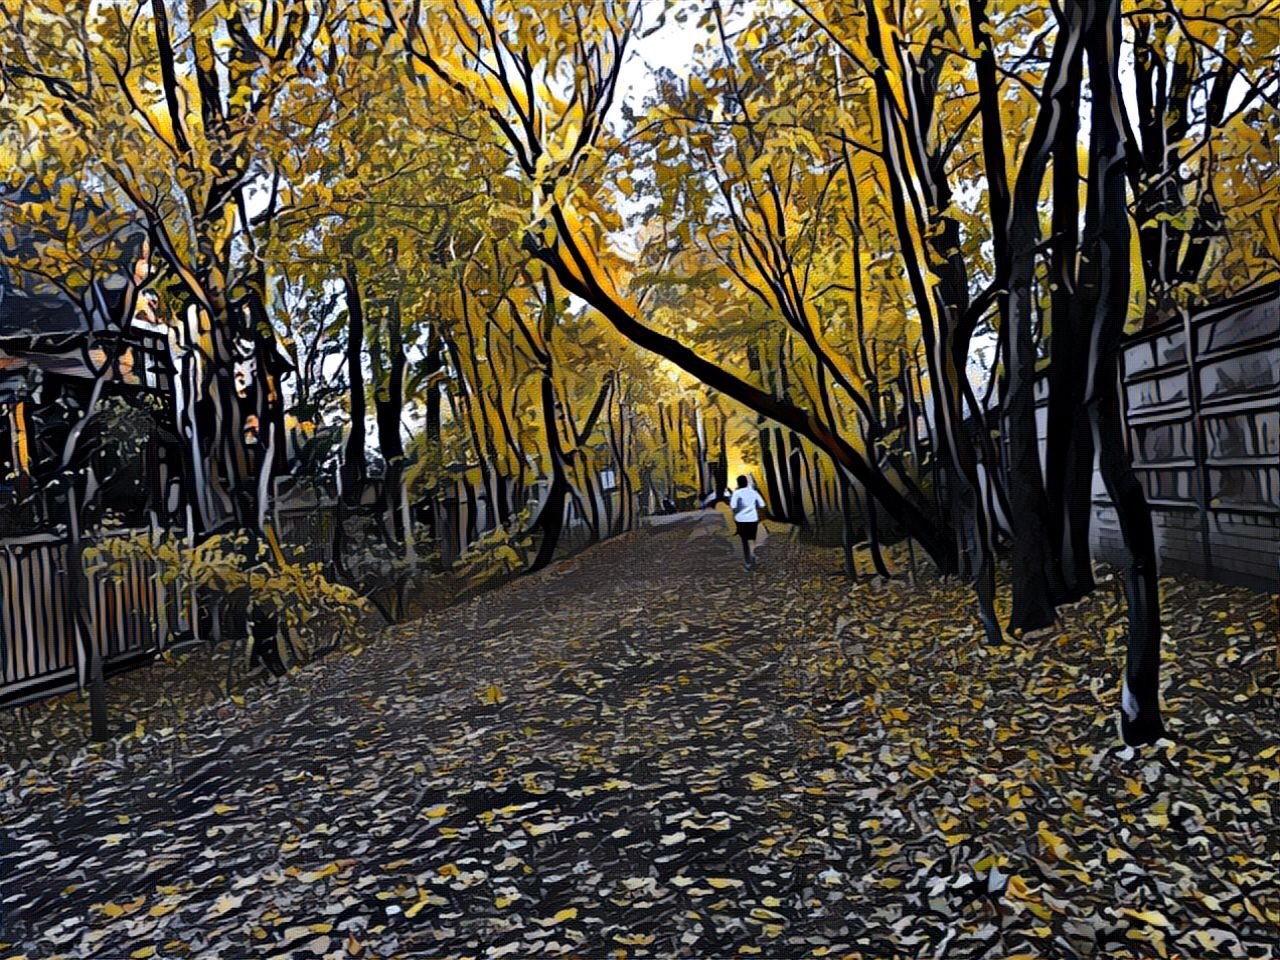
\includegraphics[width=0.75\textwidth]{TrailPic2}
\caption{\label{fig:pathB}Another nice picture of the beltway trail}
\end{figure}

\lipsum[10-11]


\chapter{First Chapter Again because it was good}

\lipsum[11-14]

\section{First Section}

\lipsum[63]

\subsection{Sub Section}

\lipsum[41-45]

\subsection{Another Sub Section with some math}

\lipsum[16-17]
Recall the Fourier\footnote{A footnote test} series formula\footnote{another footnote test \lipsum[1]}:
\[
f(x) = a_0 + \sum_{n = 1}^\infty \left( a_n \cos nx + b_n \sin nx \right)
\]
Where the Fourier coefficients $a_0$, $a_n$ and $b_n$ are defined by:
\[
a_0 = \frac{1}{2L} \int_{-L}^L f(x) dx  \qquad
a_n = \frac{1}{L}  \int_{-L}^L f(x) \cos \left( \frac{n\pi x}{L} \right) dx \qquad
b_n = \frac{1}{L}  \int_{-L}^L f(x) \sin \left( \frac{n\pi x}{L} \right) dx 
\]
\lipsum[88]

\section{Another Section with a Picture}

\lipsum[89-93]
\begin{figure}
\centering
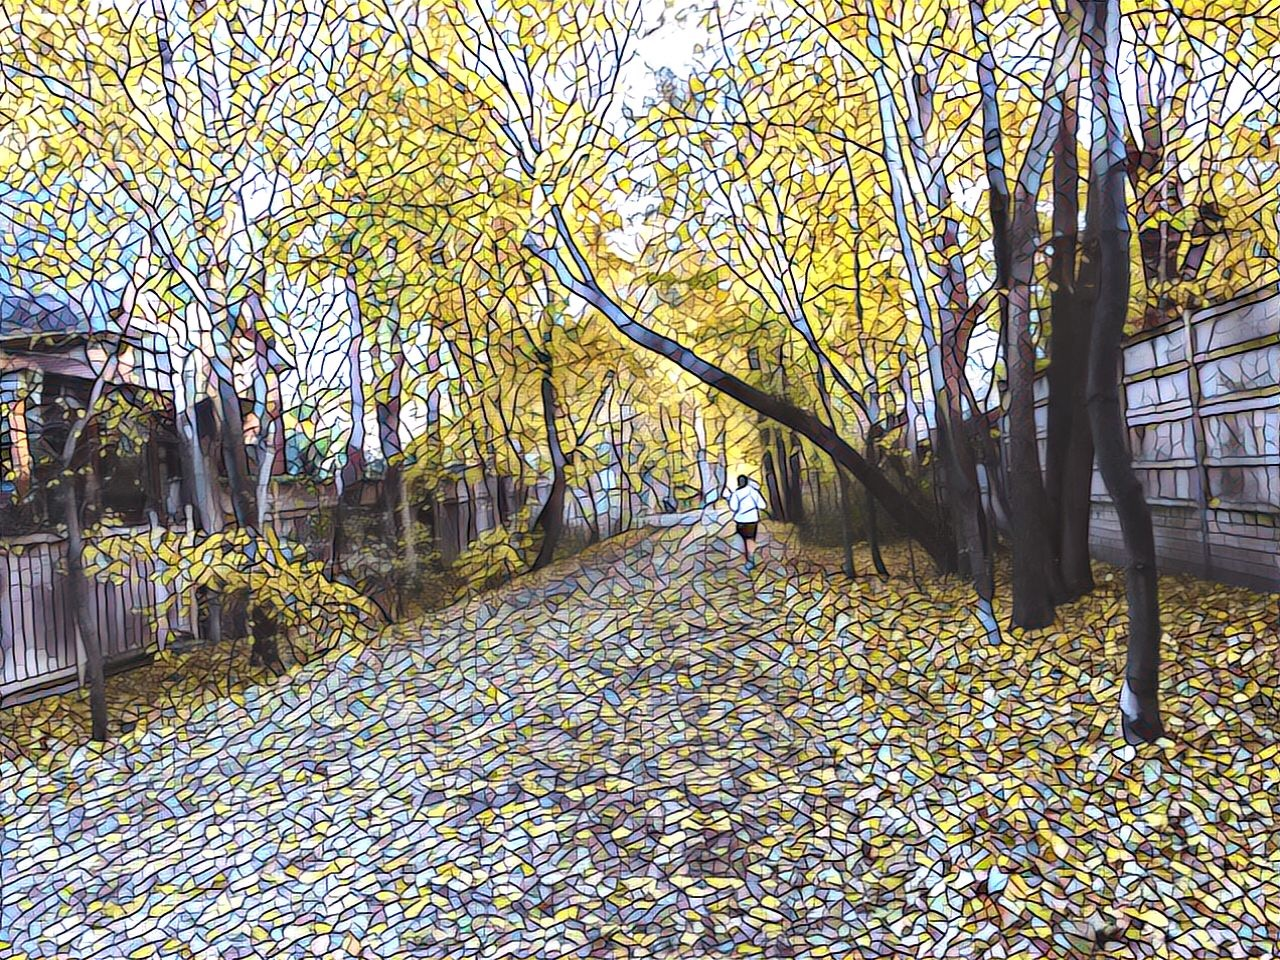
\includegraphics[width=0.5\textwidth]{TrailPic1}
\caption{\label{fig:path}A nice picture of the beltway trail}
\end{figure}

\lipsum[10-11]

\section{Another Section with more pictures}

\lipsum[12]

\begin{figure}
\centering

\includegraphics[width=0.4\textwidth]{BooksPic1}
\qquad

\includegraphics[width=0.4\textwidth]{BooksPic2}
\caption{\label{fig:path}Books and books}
\end{figure}

\lipsum[13-14]

\section{More Math}

\lipsum[15]

\[
\mathsf{Square\ Wave}(x) = \left\{ 
      \begin{array}{ll} 1, & 0 \leq x < 1 \\ 
                       -1, & 1 \leq x < 2 \end{array} \right.
\]

First we can determine $a_0$.  By inspection we can expect it to be zero, but we shall still 
figure it out for practice.  Note that $L = 1$ and we are considering the interval $[0, 2)$ instead
of $[-1, 1)$ since the function is periodic:
\begin{align*}
a_0 &= \frac{1}{2L} \int_{-L}^L f(x) dx  \\
    &= \frac{1}{2(1)} \int_{0}^{2} \mathsf{Square\ Wave}(x) dx \\
    &= \frac{1}{2} \left[ \int_0^1 (1) dx + \int_1^2 (-1) dx \right] = \frac{1}{2} \left[ \left. \vphantom{\frac{1}{2}} x\right|^1_0 - \left. \vphantom{\frac{1}{2}} x\right|^2_1 \right] \\
    &= \frac{1}{2} \left[ \vphantom{\frac{1}{2}} 1 - 0 - (2 - 1) \right] \\
    &= 0
\end{align*}

Next we shall look at $a_n$.  Again by inspection we can argue that since the function is odd that it
cosine components since those are even.  Anyways... we shall still work it out for practice.
\begin{align*}
a_n &= \frac{1}{L}  \int_{-L}^L f(x) \cos \left( \frac{n\pi x}{L} \right) dx \\
    &= \frac{1}{(1)} \int_{0}^{2} \mathsf{Square\ Wave}(x)\cos \left( \frac{n\pi x}{1} \right) dx \\ 
    &= \int_0^1 (1) \cos \left( n\pi x \right) dx + \int_1^2 (-1) \cos \left( n\pi x \right) dx \\
    &= \left. \frac{1}{n \pi} \sin \left( n\pi x \right)\right|^1_0 -  \left. \frac{1}{n \pi} \sin \left( n\pi x \right)\right|^2_1 \\
    &= \frac{1}{n \pi} \left( \vphantom{\frac{1}{2}} \sin ( n\pi) - \sin(0) \right) - \frac{1}{n \pi} \left( \vphantom{\frac{1}{2}} \sin (2n\pi) - \sin(n\pi) \right) \\
\intertext{Since $\sin(0) = 0$, $\sin ( n\pi) = 0$, and $\sin (2n\pi) = 0$ for all positive integer values of $n$, then}
a_n &= 0
\end{align*}

Now working out $b_n$...
\begin{align*}
b_n &= \frac{1}{L} \int_{-L}^L f(x) \sin \left( \frac{n\pi x}{L} \right) dx \\
    &= \frac{1}{(1)} \int_0^2 \mathsf{Square\ Wave}(x) \sin \left( \frac{n\pi x}{1} \right) dx \\
    &= \int_0^1 (1) \sin \left( n\pi x \right) + \int_1^2 (-1) \sin \left( n\pi x \right) dx \\
    &= \left. -\frac{1}{n \pi} \cos \left( n\pi x \right)\right|^1_0 + \left. \frac{1}{n \pi} \cos \left( n\pi x \right)\right|^2_1 \\
    &= -\frac{1}{n \pi} \left( \vphantom{\frac{1}{2}} \cos ( n\pi ) - \cos ( 0 ) \right) + \frac{1}{n \pi} \left( \vphantom{\frac{1}{2}} \cos(2n\pi) - \cos(n\pi) \right) \\ 
    &= \frac{1}{n \pi} \left( \vphantom{\frac{1}{2}} 1 - \cos(n\pi) - \cos(n\pi) + 1\right) \\
\intertext{Note $\cos(n\pi) = -1, 1, -1, 1, \ldots$\ which can be writen as $(-1)^n$, so then: }
b_n &= \frac{2}{n \pi} \left( \vphantom{\frac{1}{2}} 1 - (-1)^n \right) \\
    &= \frac{2}{n \pi} \left\{ \vphantom{\frac{1}{2}} 2, 0, 2, 0, \ldots \right\} \\
    &= \frac{4}{n \pi} \left\{ \vphantom{\frac{1}{2}} 1, 0, 1, 0, \ldots \right\} \\
\intertext{Therefore $b_n = 1$ for odd values of $n$ and $b_n = 0$ for even values of $n$.  To `select' just the odd numbers, we can use $2n - 1$.  So then we have:} 
b_n &= \frac{4}{(2n - 1)\pi} 
\end{align*}

And the final Fourier series is:
\[
f(x) = \frac{4}{\pi} \sum^\infty_{n = 1} \frac{1}{2n - 1} \sin \left( (2n - 1) \pi \vphantom{\frac{1}{2}} x \right)
\]

\lipsum[16-17]



\end{document}


